\section{Extraktion}
Kommen wir nun zum ersten Teil, die Extraktion. Dafür analysieren wir zunächst die Daten welche wir extrahieren werden. Die DBLP bietet dafür 2 Möglichkeiten an. Die erste ist eine Request API oder auch eine Schnittstelle an. Das heißt man kann über eine Request, also über eine Anfrage, an den Server der DBLP Daten erhalten. Es ist also Möglich eine Anfrage zustellen die alle Autoren die mit A anfangen anfragt. Für unseren Fall ist die zweite Möglichkeit besser geeignet, denn hier bekommt man ein Dump File welches dblp.xml heißt. Ein Dump File ist ein Ausdruck von dem gesamten Inhalt eines Speichers in dem Fall von einer Datenbank. Das File enthält alle Daten die die Datenbank zu dem Zeitpunkt besitzt. Da sich die Datenbank regelmäßig erweitert oder ändert, erstellt die DBLP regelmäßig neue Dump Files. Das File was benutzt wird ist vom 13.05.2020. Es kann viele Dateiformate haben, aber in diesem Fall ist es im XML-Format. Hierzu gibt es eine Dokumentation die die Formatierung des XML-Formates beschreibt. Da diese schon 'DBLP - Some Lessons Learned' heißt lässt es darauf schließen das einige Fehler bei dem ursprünglichen Design aufgetreten sind und einige Änderungen gemacht wurden. Die erste Dokumentation der DBLP ist vom 18. Juni 2009. Zu dem Zeitpunkt waren nur 532MB in der XML-Datei. Im Gegensatz da zu sind jetzt 2.806MB in der Datei also schon das 5-Fache der ursprünglichen Datei. Durch das Wachstum wurden einige Anpassungen getätigt die von der Dokumentation abweichen. Somit muss die Formatierung der Datenstrukturen an Hand der Datei selber herausgefunden werden. 

Für das Extrahieren der Daten wird dann ein Parser benötigt der die XML-Datei ausliest. Die meisten Parser lesen die Datei komplett ein und geben die XML-Daten dann aus. Da die Datei nun 2,8 GB groß ist laufen die meisten Parser an ihre grenzen. Es gibt Parser mit denen es funktionieren würde, aber in dem Fall haben wir uns bewusst dagegen entschieden. Daher wird ein eigener Parser geschrieben um dieses Problem zu umgehen. Durch die Dokumentation erfahren wir das es nur eine bestimmte Anzahl an Tags gibt die verwendet werden.
\begin{center}
	<!ELEMENT dblp (article|inproceedings| proceedings|book|incollection|phdthesis|mastersthesis|www)*>
\end{center}

Das ist ein Ausschnitt aus der Dokumentation und beschreibt alle Elemente(Tags) die auftreten können. Nach dem Testen traten auch keine anderen Elemente auf. So werden die benötigten Fähigkeiten die der Parser haben muss limitiert.

\subsection{Parser}
Um mit der Erklärung des Parsers anzufangen müssen wir erst das Dateiformat XML weiter ausführen. XML heißt Extensible Markup Language und ist eine erweiterbare Auszeichnungssprache mit deren Hilfe man Daten im Textformat speichern kann. Es funktioniert so das man mit einem Tag einem bestimmtem Element einen Namen oder eine Kategorie zuteilen kann z.b '<author> Timo Stroick </author>'. Hierbei ist Alles zusammen ein Element und das eingeklammerte 'author' ein Tag. Dabei ist darauf zu achten das man Elemente immer mit dem dazugehörigen Endtag schließen muss wie im Beispiel schon gezeigt. Eine weitere Möglichkeit ist Elemente in Elemente zu schreiben. Hier gibt es eine Besondere Regel die XML ausmacht. Denn Elemente die in anderer Elemente geschrieben sind müssen erst geschlossen werden bevor die äußeren geschlossen werden dürfen. Durch diese Regeln entsteht die Typische hierarchische Struktur des XML Dateiformats. In der dblp.xml sind alle Daten in ein Tag eingeschlossen das dblp heißt. So fängt die Datei bei <dblp> an und enden bei </dblp>. Damit sind alle wichtigen Daten zwischen den beiden Tags. 
\newpage
\begin{figure}[!htb]
	\centering
	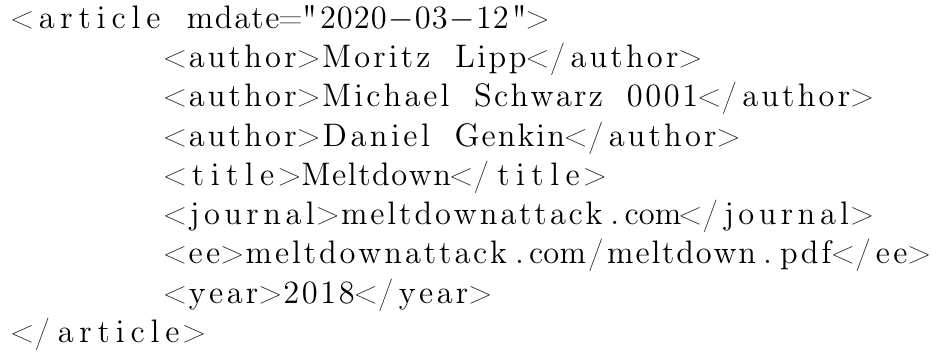
\includegraphics[width=14cm,keepaspectratio]{bilder/xmlAusschnitt}
	\caption{XML-Ausschnitt}
	Ein Beispiel Ausschnitt wie ein typischer Eintrag in der dblp.xml aussieht. Dieser wurde verkürzt und angepasst.
\end{figure}

Der Parser ist in einer eigenen Klasse. Um nun mit dem Parser anzufangen lesen wir die Daten zeilenweise in der Klasse ein um das Problem mit der Dateigröße zu umgehen. Denn würde man alles auf einmal einlesen würde der Speicher des Programms schnell voll werden und damit den Computer überlasten. Nun suchen wir in den Zeilen nach den Tags. Wenn wir einen Tag gefunden haben überprüfen wir dessen Namen und reagieren mit einem bestimmten Fall. Da wir durch die Dokumentation alle Tags kennen, die in der 2. Hierarchie auftreten können, wissen wir das nur 8 Fälle behandelt werden müssen. Somit haben wir nur 8 Methoden mit denen wir jeden Fall abdecken. Jede Methode liest weiter Tags ein bis das Endtag die Methode beendet. Das zählt natürlich auch für das dblp-Endtag welchen den Parser beendet. Die nun eingelesenen Elemente in der 3. Hierarchie sind die Daten des entsprechenden Elements wie zum Beispiel bei 'article' könnte es der Autor sein der eingelesen wird. Die Daten werden nun in eine weitere Klasse übergeben und dort den richtigen Entitäten zugewiesen, denn die 8 Elemente der XML-Datei sind nicht die Entitäten die wir in der Datenbank benutzen. Wir wollen die Datenbank so Allgemeingültig halten wie möglich. Zum Schluss wird in der Insert Klasse die Daten nur noch in die Datenbank eingefügt. Somit sind alle Daten von einem Element gespeichert und so das man den Arbeitsspeicher erneut benutzen kann. Damit sorgen wir dafür das nur ein Element gleichzeitig bearbeitet wird und kein Speicherüberlauf auftritt. Alle Klassen folgen dem Single Responsibility Principle dieses besagt das jede Klasse nur eine Aufgabe verfolgt. Dem nach extrahiert die Parser-Klasse die Daten , die DBParser-Klasse teilt die Daten in die Entitäten auf und die Insert-Klasse fügt die Daten in die Datenbank ein. So ist das Programm besser wartbar und es gibt ein sauberes Programmbild ab.
\newpage
\begin{figure}[!htb]
	\centering
	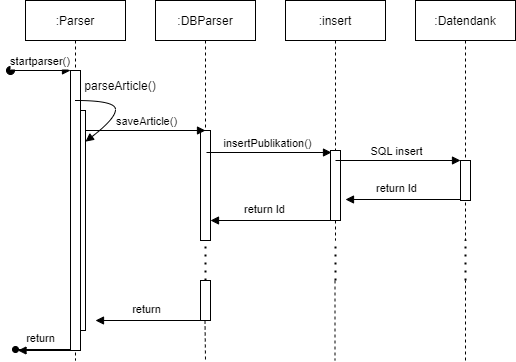
\includegraphics[width=10cm,keepaspectratio]{bilder/SequenzDiagramParser}
	\caption{Sequenzdiagramm-Auschnitt}
	\label{fig:sequenzdiagramm}
\end{figure}

In Abbildung \ref{fig:sequenzdiagramm} sehen wir einen Typischen Programmablauf vom Parser. In diesem Beispiel Ablauf wird ein 'article' Element eingelesen. Zu nächst wird die Parser-Klasse mit der startParser-Funktion in der Main-Methode aufgerufen und liest einen Tag nach dem anderen bis er auf einen Treffer stößt. In diesem Fall ist es das Tag 'article' ein Treffer. Nun wird die parseArticle-Methode in der selben Klasse aufgerufen. In der Methode werden nun die weiter folgenden Elemente ausgelesen und deren Daten zwischengespeichert. Dies geschieht solange bis das Endtag von 'article' wieder eingelesen wird. Jetzt werden alle Daten an die saveArticle-Methode der DBParser-Klasse übergeben. In dieser Klasse werden nun die Daten an die Datenbank angepasst. Denn in der Datenbank gibt es keine Entität die Artikel heißt. Das wird erst im nächsten Abschnitt erklärt. Im Allgemeinen wird der Artikel dann in Publikation, Autoren, elektronische Version und Fachzeitschrift zerteilt und noch in die Beziehungen zwischen diesen Entitäten. Da die Daten nun richtig zerlegt sind werden sie an die Insert-Klasse übergeben. Das geschieht über die insertPublikation-Methode. Jetzt haben wir alle Daten und haben sie richtig zugewiesen. Daraufhin werden sie mit SQL in eine Postgres Datenbank gespeichert. Postgres ist ein freies objektrelationales Datenbankmanagementsystem (ORDBMS) und und basiert auf SQL. SQL bedeutet Structured Query Language also Strukturierte Abfragesprache und stellt einen Standard für relationale Datenbanken da. Es gibt viele SQL-Datenbanken wie zum Beispiel Amazon DynamoDB, IBM DB2, MongoDB, PostgresSQL und viele weitere. PostgresSQL verwenden wir da es zunächst eine freie Open-Source Datenbank ist in der keine Lizenzen benötigt wird. Dazu hält sie weitestgehend die SQL-Standards und Normen ein. Diese brauchen wir auch um die Aufgabe ordentlich zu erfüllen. In den Methoden ist nämlich drauf zu achten das nur triviale SQL Befehle benutzt werden und keine Speziellen Befehle eines bestimmten Datenbank Typs. Deshalb beschränke ich mich auf Insert-Befehle und Select-Abfragen um auf keinen bestimmten Datenbank Typen angewiesen zu sein. Schlussendlich gebe ich den Primärschlüssel der Publikation zurück um die Beziehungen zwischen den Entitäten in der Datenbank einzutragen. Wenn nun die saveArticle-Methode zu ende läuft und sich erfolgreich beendet, sucht die startparser-Methode nach dem nächsten Tag. So wird jedes Element nacheinander in die Datenbank eingespeichert bis das Endtag von dblp eingelesen wird.

\subsection{Datenbank}
Zur Erstellung der Datenbank analysieren wir zunächst die Daten. Die DBLP gibt uns schon mit diesen 8 Tags (article, inproceedings, proceedings, book, incollection, phdthesis, mastersthesis, www) einen groben Überblick. Nur diese Tags sind noch nicht in dem relationalen Datenbank Format. Deshalb werden diese Tags nochmal in kleinere Entitäten zerteilt. Zunächst werden wir die Begriffe ein wenig klarer stellen. Ein 'article' ist ein Artikel oder auch eine Publikation in einer Fachzeitschrift. 'proceedings' ist in diesem Zusammenhang eine Konferenz die gehalten wurde und dazu passend sind 'inproceedings' Puplikationen die zu dieser Konferenz gehören. 'incollection' ist eine Publikation in einem Buch. 'book' dazu ist das ein Buch mit einem Autor. 'masterthesis' ist eine Publikation die an einer Universität geschrieben wurde. Fast das selbe ist die 'phdthesis' diese besitzt nur zusätzliche Bucheigenschaften. Schlussendlich haben wir nur noch das Tag 'www' hier kann ein Autor eine Homepage besitzen. Da in der DBLP Bücher sind die mehrere ISBN's haben muss eine extra Entität für die ISBN erstellt werden. Das gleiche zählt für die elektronische Version, denn diese existiert für die meisten Entitäten mehrfach. Daraus ergeben sich dann diese Entitäten Autor, Publikation, Homepage, Konferenz, Fachzeitschrift, Buch, elektronische Version, ISBN und deren Beziehungen. Hiermit wird dann ein ER Modell modelliert und an die entsprechenden Entitäten und Beziehungen angepasst. 

\newpage
\subsubsection{ER-Modell}
\begin{figure}[!htb]
	\centering
	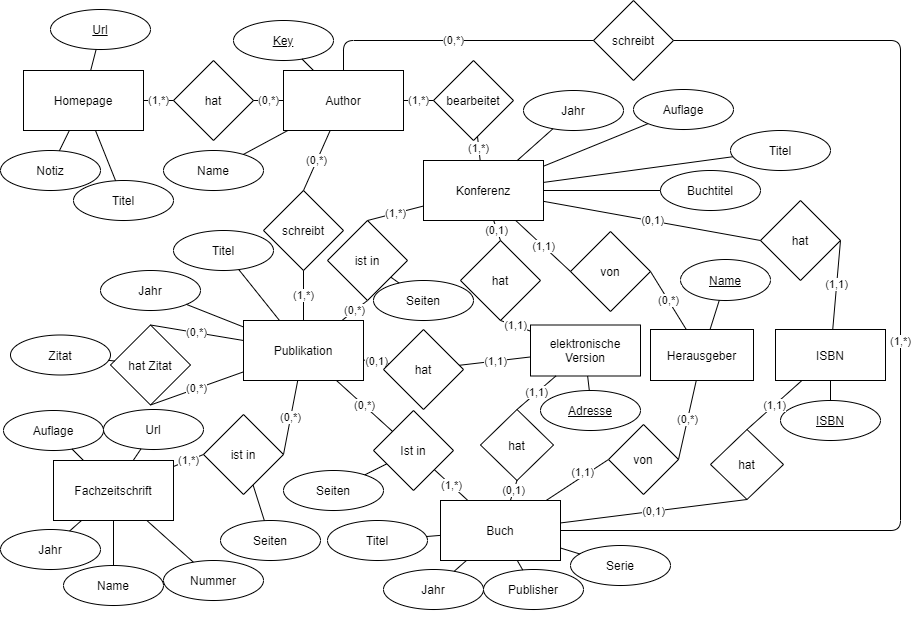
\includegraphics[width=14cm,keepaspectratio]{bilder/ER-Modell}
	\caption{ER-Modell}
	\label{fig:er-modell}
\end{figure}
Das ER-Modell veranschaulicht die Beziehungen zwischen den Entitäten. Die Entitäten sind hier die Rechtecke. Die Attribute sind Kreise und direkt mit den Entitäten verbunden zu denen sie gehören. Beziehungen werden durch Rauten dargestellt und verbinden immer 2 Entitäten oder nur eine Entität mit sich selber wie zusehen bei der Beziehung hat-Zitat. Ein Zitat verbindet eine Publikation mit der Publikation die zitiert wurde. Man sieht auch das Beziehungen Attribute haben können, denn es gibt Fälle wo dieses Attribut zu keinem von beiden passt. Das Attribut passt nur wenn beide in Beziehung stehen. Wenn man sich die Relation zwischen Publikation und Buch an sieht, hat sie das Attribut Seiten. Dies macht keinen Sinn nur im einzelnen Zusammenhang, da Seiten allein in einer Publikation ohne Buch keinen Anhaltspunkt besitzt. Andersherum kann ein Buch mehrere Publikationen beinhalten und deshalb nicht verschiedene Seitenangaben für verschiedene Publikationen speichern. Somit macht die Angabe von Seiten nur Sinn in der Beziehung der beiden Entitäten.

Dieses Modell müssen wir nun umwandeln. Da wir in der Datenbank nur Tabellen anlegen können müssen wir dieses ER-Modell in die Form von Tabellen bringen. Diese Form ist dann das Relationale Schema. Dieses Schema beschreibt genau das Gleiche, wie das ER-Modell.

\subsubsection{Relationales Schema}

\begin{figure}[!htb]
	\centering
	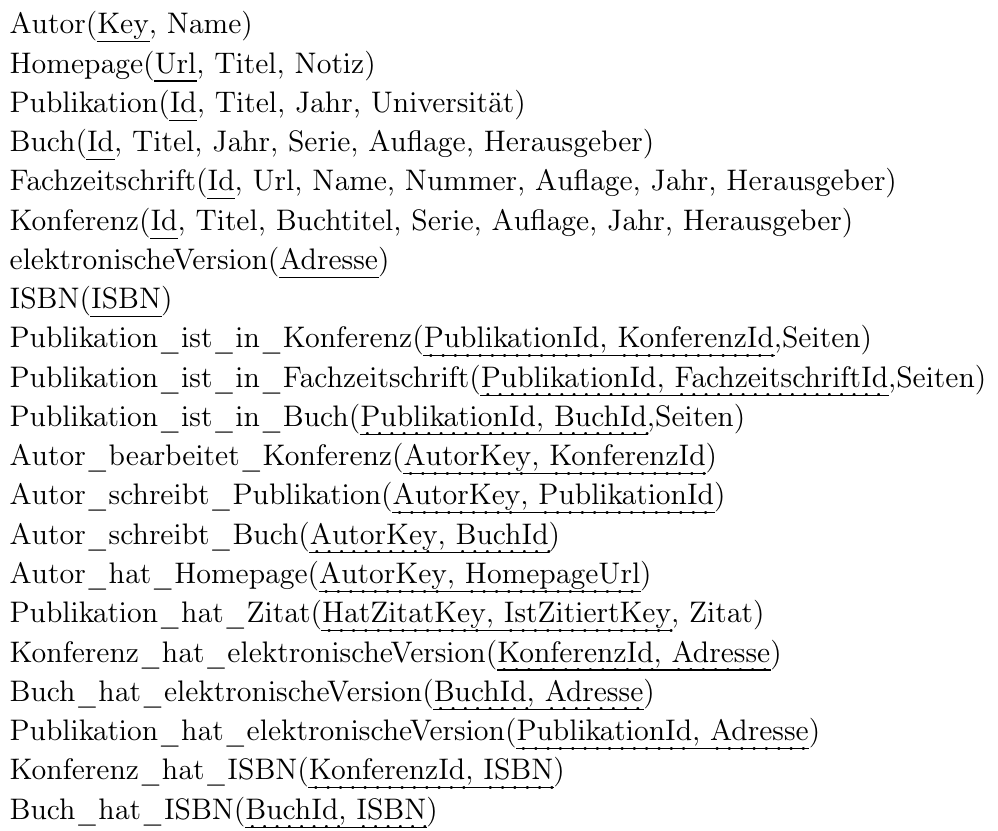
\includegraphics[width=12cm,keepaspectratio]{bilder/relationalesSchema}
	\caption{Relationales Schema}
	\label{fig:relationalesSchema}
\end{figure}

Das ist nun das ER-Modell genau übertragen ins Relationale Schema. Der erste Name ist der Name der Tabelle und alle Namen in der Klammer sind die Attribute in der Tabelle. Hier sieht man das auch Beziehungen zwischen den Entitäten eine eigene Tabelle bekommen. Diese sorgen dafür das Entitäten mit einander verbunden werden. Die unterstrichenen Attribute stellen die Primärschlüssel da. Primärschlüssel sind Attribute womit man die Daten dieser Entität genau unterscheiden kann wie zum Beispiel die Studierendennummer die sich bei jedem Studenten unterscheidet. Gibt es keine eindeutige Eigenschaft so erstellen wir einen künstlichen Schlüssel. In dem Fall heißen alle künstlichen Schlüssel Id. Diese Id wird mit jeder Erstellung eines neuen Eintrags erhöht. Die unterpunkteten Attribute sind Fremdschlüssel. Diese Schlüssel sind Primärschlüssel aus anderen Tabellen. Für das Erste wird in dem Schema jede Beziehung als Tabelle mit 2 Fremdschlüsseln erstellt. Die Schlüssel kommen aus den Entitäten die sie verbinden. Damit stellen sie eine eindeutige Verbindung zwischen Entitäten her. Da hier noch überflüssige Tabellen enthalten sind werden die Tabellen verschmolzen.

\newpage
\subsubsection{Verschmolzenes relationale Schema}

\begin{figure}[!htb]
	\centering
	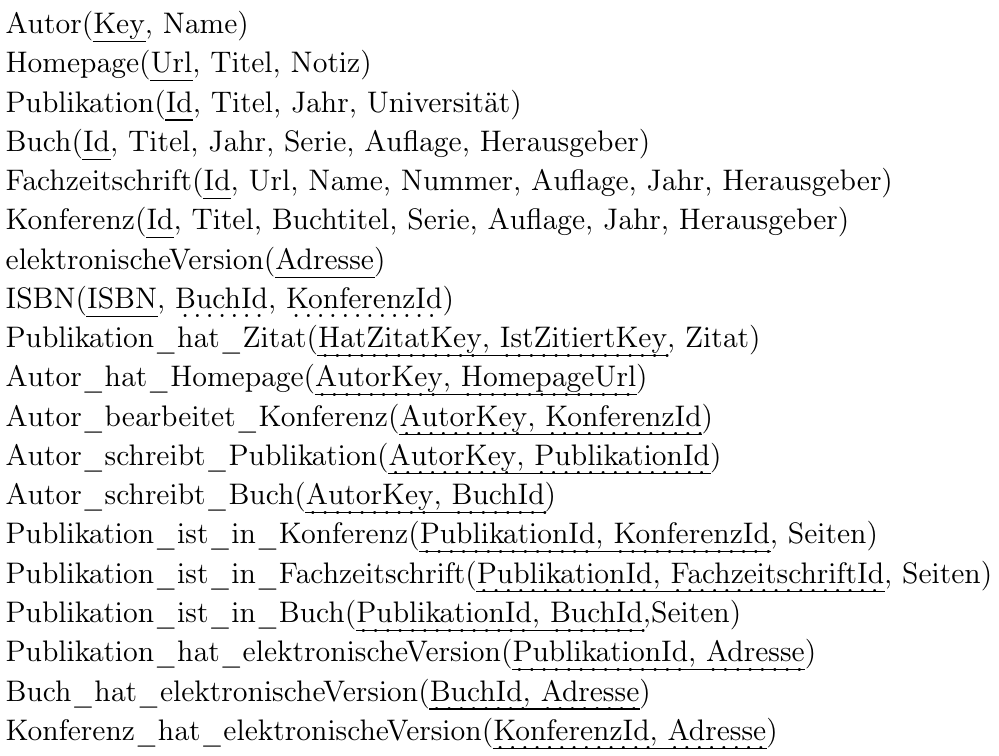
\includegraphics[width=13cm,keepaspectratio]{bilder/verschmolzenesRelationaleSchema}
	\caption{Verschmolzenes Relationale Schema}
	\label{fig:verschmolzenesrelationalesSchema}
\end{figure}

Das ist nun das verschmolzene relationale Schema. Man sieht das einige Tabellen nun anders aussehen. Zum Beispiel verschwindet die Tabelle Buch-hat-ISBN ganz, denn der Primärschlüssel vom Buch steht nun direkt in der ISBN da es nur ein Buch für eine ISBN geben kann. Das selbe passiert mit Konferenz und ISBN. Dies ist eine N zu 1 Beziehung gewesen, da Fälle auftreten wo Bücher mehrere ISBN's haben. Die meisten anderen Beziehungen sind N zu M Relationen wie zum Beispiel Autor und Publikation. Jeder Autor kann mehrere Publikationen schreiben und das ganze auch andersherum, denn Publikationen können von mehreren Autoren geschrieben werden. Diese Relationen können nicht verschmolzen werden. Der letzte Fall wäre eine 1 zu 1 Relation, aber die kommt in diesem Modell nicht vor. Ein typisches Beispiel ist eine Person und ihr Ausweis, denn eine Person hat nur einen Ausweis und ein Ausweis darf nur einer Person gehören.

\subsubsection{Normalisierung}

Um Redundanzen und Fehler zu verhindern gibt es Normalformen. Je höher die Stufe der Normalform desto weniger Anomalien können auftreten. Anomalien sind Erscheinungen die denn Umgang mit der Datenbank erschweren oder sogar ganz stoppen. Es können Daten gelöscht werden die nicht gelöscht werden sollten. Namen können verschieden sein die eigentlich gleich seien sollten.  Insgesamt gibt es 3 Anomalien die einfach durch die Normalisierungen verhindert werden können.

Die Einfüge-Anomalie ist eine Anomalie die beim einfügen von Daten in der Datenbank auftritt. Es kann passieren das man einen Primärschlüssel hat der 2 Schlüssel umfasst. Da das Einfügen nun verlangt das beide Primärschlüssel vorhanden sind führt dies zu Schwierigkeiten oder auch zu Fehlern.

Beispiel:
\begin{figure}[!htb]
	\centering
	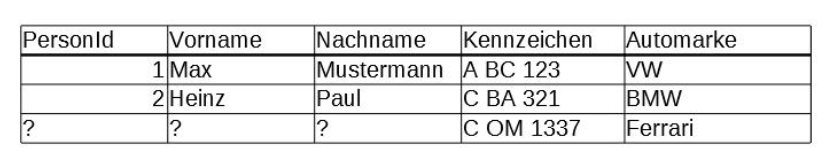
\includegraphics[width=13cm,keepaspectratio]{bilder/KFZBeispiel}
	\caption{Einfüge-Anomalie Beispiel}
	\label{fig:kfzbeispiel}
\end{figure}

Wir gehen davon aus das die Schlüssel PersonId und Kennzeichen zusammen den Primärschlüssel ergeben, da eine Person mehrere Autos haben kann. Will man jetzt ein neues Auto einfügen für das zu Problemen, denn ein Auto kann in diesem Beispiel nicht ohne eine Person existieren. Wie hier zusehen ist der Ferrari ohne Person und hat damit keinen vollständigen Primärschlüssel. Die würde auch anderes herum zu Problemen führen da eine Person auch nicht ohne ein Auto existieren kann. Somit haben wir eine Einfüge-Anomalie. 

Die Änderungs-Anomalie tritt beim ändern von Daten in der Datenbank auf. Wenn wir viele redundante Daten in einer Tabelle haben und einen Namen ändern wollen, tritt diese Anomalie auf wenn wir diesen einen Namen an vielen Stellen ändern müssen. Wobei hier eigentlich eine Änderung reichen sollte.

Beispiel:
\begin{figure}[!htb]
	\centering
	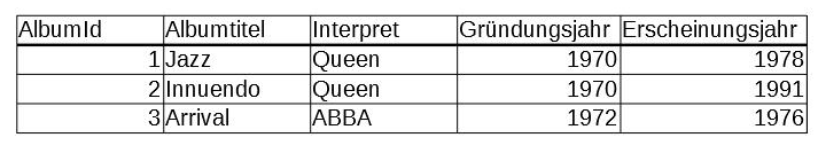
\includegraphics[width=13cm,keepaspectratio]{bilder/AlbumBeispiel}
	\caption{Lösch- und Änderungs-Anomalie Beispiel}
	\label{fig:albumbeispiel}
\end{figure}

Hier ist der Primärschlüssel die AlbumId. Die Probleme treten hier auf wenn man denn Namen von Queen ändern würde. Normalerweise sollte eine Änderung reichen um ein Attribut-wert zu ändern. In diesem Fall müssten wir jedes Album durch gehen und da die Namen anpassen. Dieser extra Aufwand ist die Änderungs-Anomalie.

Die Lösch-Anomalie entsteht durch das löschen von Daten aus der Datenbank. Wenn wir zwei unabhängige Daten löschen wollen und durch denn Aufbau beide Informationen löschen, haben wir eine Anomalie. Das Löschen sollte nur die Daten löschen die auch beabsichtigt sind zu löschen. 

Beispiel:
Hier nehmen wir das Beispiel aus Abbildung \ref{fig:albumbeispiel}. Der Primärschlüssel ist immer noch AlbumId. Nun wollen wir nichts mehr ändern sondern löschen. Wenn wir jetzt das Album Arrival von ABBA löschen, würden wir damit auch direkt die Band ABBA löschen. Obwohl wir nur beabsichtigt hatten das Album zu löschen.

Diese Anomalien werden durch die Normalformen alle beseitigt. Damit gucken wir uns die verschieden Stufen der Normalformen an.

Die erste Normalform besagt das jedes Attribut atomar sein soll. Damit ist gemeint das man Daten zerkleinern soll die auch im einzelnen Aspekt eine Gewichtung haben zum Beispiel Adressen. Adressen kann man als eins zusammen schreiben, aber Atomar wäre sie erst wenn man sie in Straße, PLZ, Hausnummer und Stadt einteilt. Diese Einteilung verschafft nachher Vorteile. Man kann einfacher nach Leuten suchen die alle in einer Stadt wohnen. Ohne diese atomaren Attribute müsste man die Adresse erst zerlegen und dann könnte man erst suchen. Diese Regel wird leider in unserer Datenbank gebrochen da die Namen von Autoren nicht in Vor- und Nachnamen geteilt sind. 

In der DBLP sind die Autoren als ein ganzer Name gespeichert. Wären sie im voraus getrennt gewesen würden wir hier die Namen in Vor- und Nachname teilen. Namen zu trennen ist eine Aufgabe für sich. Namen wie Jürgen von der Lippe oder Angela Dorothea Merkel haben schon verschiedene Trennungsmöglichkeiten. Aber diese zu verallgemeinern, ist eine große Aufgabe. Dazu kommen dann Namen aus Ostasien die wiederum Vor-und Nachname andersherum aufschreiben, denn hier kommt der Familien Name zuerst. Somit ist dies aufzuteilen zu viel für diese Bachelorarbeit. Deshalb nehmen wir an das Namen Atomar sind.

Für die zweite Normalform muss sie erst mal in der 1. Normalform sein und dazu darf kein Attribut, welches auch kein Primärschlüssel ist, eine Teilmenge in der Tabelle besitzen die von dem Attribut abhängig ist. Also Attribute müssen vollständig von einem Primärschlüssel abhängig sein und nicht nur halb. Hier durch wird auch die Einfüge-Anomalie gelöst da es nun keine 2 einzelne Entitäten mehr gibt die in eine Tabelle zusammen gefügt sind. Um das nochmal zu verdeutlichen hier ein Beispiel.

\begin{small}
	Person(\uline{Id}, Name, Nachname, Kennzeichen, Automarke, Autotyp)
\end{small}

In dieser Tabelle wäre Kennzeichen ein Primärschlüssel von Automarke und Autotyp und damit hat ein Nichtprimärattribut eine Teilmenge von Attributen die von ihm abhängig ist. Zwar gehört das Auto dieser Person, aber es wäre nur vollständig abhängig von der Kombination der beiden Attribute Id und Kennzeichen. Damit ist diese Tabelle nicht in der zweiten Normalform dafür müssen die Tabellen so aussehen.

\begin{small}
	Person(\uline{Id}, Name, Nachname, \dotuline{Kennzeichen})\newline
	Auto(\uline{Kennzeichen}, Automarke, Autotyp)
\end{small}

Kommen wir nun zur dritten Normalform zunächst muss die Tabelle in der 2 Normalform sein und dann darf kein Nichtprimärschlüssel transitiv von einem Schlüsselkandidaten abhängen. Schlüsselkandidaten sind Attribute die als Primärschlüssel Infrage kommen. Durch diese Normalform werden direkt 2 Anomalien beseitigt, die Änderung-Anomalie und die Lösch-Anomalie. Um dies Klar zustellen nehmen wir ein Album als Beispiel.

\begin{small}
	Album(\uline{Id}, Albumtitel, Interpret, Gründungsjahr, Erscheinungsjahr)
\end{small}

Hier wäre Gründungsjahr Transitiv über Interpret abhängig und würde somit die Regel brechen also muss der Interpret eine eigene Entität werden. Damit sehen die Tabellen dann so aus.

\begin{small}
	Album(\uline{Id}, Albumtitel, Erscheinungsjahr, Interpret)\newline
	Künstler(\uline{Interpret}, Gründungsjahr)
\end{small}

Die Tabelle ist in der dritten Normalform, wenn man davon ausgeht das der Interpret eindeutig ist ansonsten wird noch ein künstlicher Schlüssel eingefügt. 

In der dritten Normalform sind nun alle Anomalien beseitigt. Das sind die Grundeigenschaften die eine Datenbank erfüllen muss. Unsere Datenbank erfüllt alle Kriterien der dritten Normalform, wenn man davon ausgeht das Namen ungetrennt schon atomar sind, falls nicht wäre sie in der nullten Normalform.

\subsection{Datendefinition in der Datenbank}

Nun haben wir die gesamten theoretischen Teil unsere Datenbank beschrieben. Jetzt kommen wir zur Praxis. Hierzu verwenden wir DDL das heißt ausgeschrieben Data Definition Language und ist ein Teil von SQL. Diese Sprache wird verwendet um die Datenstruktur die wir uns Theoretisch aufgebaut haben in der Datenbank anzulegen. Also alle Tabellen, Beziehungen, Datentypen und vieles mehr. 

\begin{figure}[!htb]
	%\includegraphics[width=13cm,keepaspectratio]{bilder/DDLBeispiel}
	\oranget{CREATE TABLE} AUTORSCHREIBTBUCH( \newline
	KEY \purplet{VARCHAR(100)} \oranget{NOT NULL},\newline
	ID \purplet{INTEGER}        \oranget{NOT NULL},\newline
	\oranget{PRIMARY KEY}(KEY,ID),\newline
	\oranget{FOREIGN KEY}(KEY) \oranget{REFERENCES} AUTOR(KEY)\newline
	\oranget{ON DELETE} CASCADE \oranget{ON UPDATE} CASCADE,\newline
	\oranget{FOREIGN KEY}(ID) \oranget{REFERENCES} BUCH(ID)\newline
	\oranget{ON DELETE} CASCADE \oranget{ON UPDATE} CASCADE);\newline
	\caption{DDL Ausschnitt}
	\label{fig:ddlbeispiel}
\end{figure}

Das ist ein Typischer SQL Ausschnitt und hier wird gerade die Tabelle Autor-schreibt-Buch erstellt. Dazu ist zu beachten das SQL nicht case sensitive ist also achtet die Sprache nicht auf Groß- und Kleinschreibung. Wie man hier sieht wird erst der Create-Befehl benutzt so das man eine Tabelle namens AUTORSCHREIBTBUCH erstellt und in der dahinterliegenden Klammer kommt die Tabellenstruktur. Hier werden erst die beiden Attribute Key und ID erstellt. Hinter den jeweiligen Namen kommen die Datentypen. In unserem Varchar und Integer. Varchar steht für eine variable Zeichenkette mit einem Maximum an Zeichen. Variabel ist sie da sie nicht immer die maximale Anzahl als Speicher einnimmt. Integer steht für eine Ganzzahl. Fasst alle Attribute sind in Varchar gespeichert da die DBLP nicht genormt ist. Viele Werte die eigentlich ein Integer wären werden durch Ausnahmen wieder zu Varchar zum Beispiel gibt es bei Büchern das Attribut Auflage(Volume). Durchweg werden hier Ganzzahlen verwendet die Auflagen beschreiben, aber manche Auflagen sind mit langen Komplizierten Zeichenketten beschrieben was Integer wieder hinfällig macht. Deshalb sind nur die künstlichen Schlüssel vom Typ Integer. Diese Tabelle ist die Relation zwischen Autor und Buch. Deshalb sind beide Attribute Fremdschlüssel(Foreign Key). Erst wird der Fremdschlüssel als ein solcher markiert und danach referenzieren wir ihn auf die Tabelle mit dem Attribut zu dem es gehört. Dabei spielt es keine Rolle ob der Fremdschlüssel den selben Namen hat, mit dem Primärschlüssel den er repräsentiert. So könnten wir auch Fremdschlüssel umbenennen und trotzdem nachher auf den Richtigen Primärschlüssel verweisen.
Man könnte zum Beispiel ID auf BuchId ändern dazu müsste man nur die zwei ID's umbenennen, aber dabei nicht die Referenz ändern.

Unter dem Foreign-Key-Befehl stehen noch optionale Eigenschaften zu Fremdschlüsseln. Hiermit wird beschrieben was passiert bei einer Änderung oder Löschung von dem Primärschlüssel in der referenzierten Tabelle. Es gibt 5 Möglichkeiten die man Einstellen kann.

NO ACTION - Hier wird nichts mit der Tabelle getan. Da dann aber ein Fremdschlüssel auf einen Datensatz verweist wird ein Fehler geworfen. Dies ist auch die Standard Einstellung wenn man keine Option wählt.

RESTRICT - Es wird verboten den verwiesenen Primärschlüssel zu löschen.

CASSCADE - Der Tabellen Eintrag wird gelöscht/geändert, falls der verwiesene Primärschlüssel gelöscht wird oder sich ändert.

SET NULL - Der Fremdschlüssel wird auf Null gesetzt, wenn der verwiesene Primärschlüssel gelöscht wird oder sich ändert.

SET DEFAULT - Wie bei SET NULL nur hier wird der Fremdschlüssel auf den voreingestellten Standardwert gesetzt.

In unserem Fall benutzen wir beide male CASSCADE da dies eine Relations Tabelle ist und diese die Änderungen und Löschungen mit übernehmen soll. Da diese Tabelle nur die Beziehung darstellt und keine wirklichen Daten besitzt, geschehen hiermit keine Löschungen oder Änderungen die Fehler erzeugen könnten.


\subsection{Daten einfügen}

Nun befüllen wir die Datenbank mit den Daten die wir schon mit dem DBParser angepasst haben.












